% Options for packages loaded elsewhere
% Options for packages loaded elsewhere
\PassOptionsToPackage{unicode}{hyperref}
\PassOptionsToPackage{hyphens}{url}
\PassOptionsToPackage{dvipsnames,svgnames,x11names}{xcolor}
%
\documentclass[
  letterpaper,
  DIV=11,
  numbers=noendperiod]{scrartcl}
\usepackage{xcolor}
\usepackage{amsmath,amssymb}
\setcounter{secnumdepth}{-\maxdimen} % remove section numbering
\usepackage{iftex}
\ifPDFTeX
  \usepackage[T1]{fontenc}
  \usepackage[utf8]{inputenc}
  \usepackage{textcomp} % provide euro and other symbols
\else % if luatex or xetex
  \usepackage{unicode-math} % this also loads fontspec
  \defaultfontfeatures{Scale=MatchLowercase}
  \defaultfontfeatures[\rmfamily]{Ligatures=TeX,Scale=1}
\fi
\usepackage{lmodern}
\ifPDFTeX\else
  % xetex/luatex font selection
\fi
% Use upquote if available, for straight quotes in verbatim environments
\IfFileExists{upquote.sty}{\usepackage{upquote}}{}
\IfFileExists{microtype.sty}{% use microtype if available
  \usepackage[]{microtype}
  \UseMicrotypeSet[protrusion]{basicmath} % disable protrusion for tt fonts
}{}
\makeatletter
\@ifundefined{KOMAClassName}{% if non-KOMA class
  \IfFileExists{parskip.sty}{%
    \usepackage{parskip}
  }{% else
    \setlength{\parindent}{0pt}
    \setlength{\parskip}{6pt plus 2pt minus 1pt}}
}{% if KOMA class
  \KOMAoptions{parskip=half}}
\makeatother
% Make \paragraph and \subparagraph free-standing
\makeatletter
\ifx\paragraph\undefined\else
  \let\oldparagraph\paragraph
  \renewcommand{\paragraph}{
    \@ifstar
      \xxxParagraphStar
      \xxxParagraphNoStar
  }
  \newcommand{\xxxParagraphStar}[1]{\oldparagraph*{#1}\mbox{}}
  \newcommand{\xxxParagraphNoStar}[1]{\oldparagraph{#1}\mbox{}}
\fi
\ifx\subparagraph\undefined\else
  \let\oldsubparagraph\subparagraph
  \renewcommand{\subparagraph}{
    \@ifstar
      \xxxSubParagraphStar
      \xxxSubParagraphNoStar
  }
  \newcommand{\xxxSubParagraphStar}[1]{\oldsubparagraph*{#1}\mbox{}}
  \newcommand{\xxxSubParagraphNoStar}[1]{\oldsubparagraph{#1}\mbox{}}
\fi
\makeatother


\usepackage{longtable,booktabs,array}
\usepackage{calc} % for calculating minipage widths
% Correct order of tables after \paragraph or \subparagraph
\usepackage{etoolbox}
\makeatletter
\patchcmd\longtable{\par}{\if@noskipsec\mbox{}\fi\par}{}{}
\makeatother
% Allow footnotes in longtable head/foot
\IfFileExists{footnotehyper.sty}{\usepackage{footnotehyper}}{\usepackage{footnote}}
\makesavenoteenv{longtable}
\usepackage{graphicx}
\makeatletter
\newsavebox\pandoc@box
\newcommand*\pandocbounded[1]{% scales image to fit in text height/width
  \sbox\pandoc@box{#1}%
  \Gscale@div\@tempa{\textheight}{\dimexpr\ht\pandoc@box+\dp\pandoc@box\relax}%
  \Gscale@div\@tempb{\linewidth}{\wd\pandoc@box}%
  \ifdim\@tempb\p@<\@tempa\p@\let\@tempa\@tempb\fi% select the smaller of both
  \ifdim\@tempa\p@<\p@\scalebox{\@tempa}{\usebox\pandoc@box}%
  \else\usebox{\pandoc@box}%
  \fi%
}
% Set default figure placement to htbp
\def\fps@figure{htbp}
\makeatother





\setlength{\emergencystretch}{3em} % prevent overfull lines

\providecommand{\tightlist}{%
  \setlength{\itemsep}{0pt}\setlength{\parskip}{0pt}}



 


\KOMAoption{captions}{tableheading}
\makeatletter
\@ifpackageloaded{tcolorbox}{}{\usepackage[skins,breakable]{tcolorbox}}
\@ifpackageloaded{fontawesome5}{}{\usepackage{fontawesome5}}
\definecolor{quarto-callout-color}{HTML}{909090}
\definecolor{quarto-callout-note-color}{HTML}{0758E5}
\definecolor{quarto-callout-important-color}{HTML}{CC1914}
\definecolor{quarto-callout-warning-color}{HTML}{EB9113}
\definecolor{quarto-callout-tip-color}{HTML}{00A047}
\definecolor{quarto-callout-caution-color}{HTML}{FC5300}
\definecolor{quarto-callout-color-frame}{HTML}{acacac}
\definecolor{quarto-callout-note-color-frame}{HTML}{4582ec}
\definecolor{quarto-callout-important-color-frame}{HTML}{d9534f}
\definecolor{quarto-callout-warning-color-frame}{HTML}{f0ad4e}
\definecolor{quarto-callout-tip-color-frame}{HTML}{02b875}
\definecolor{quarto-callout-caution-color-frame}{HTML}{fd7e14}
\makeatother
\makeatletter
\@ifpackageloaded{caption}{}{\usepackage{caption}}
\AtBeginDocument{%
\ifdefined\contentsname
  \renewcommand*\contentsname{Table of contents}
\else
  \newcommand\contentsname{Table of contents}
\fi
\ifdefined\listfigurename
  \renewcommand*\listfigurename{List of Figures}
\else
  \newcommand\listfigurename{List of Figures}
\fi
\ifdefined\listtablename
  \renewcommand*\listtablename{List of Tables}
\else
  \newcommand\listtablename{List of Tables}
\fi
\ifdefined\figurename
  \renewcommand*\figurename{Figure}
\else
  \newcommand\figurename{Figure}
\fi
\ifdefined\tablename
  \renewcommand*\tablename{Table}
\else
  \newcommand\tablename{Table}
\fi
}
\@ifpackageloaded{float}{}{\usepackage{float}}
\floatstyle{ruled}
\@ifundefined{c@chapter}{\newfloat{codelisting}{h}{lop}}{\newfloat{codelisting}{h}{lop}[chapter]}
\floatname{codelisting}{Listing}
\newcommand*\listoflistings{\listof{codelisting}{List of Listings}}
\makeatother
\makeatletter
\makeatother
\makeatletter
\@ifpackageloaded{caption}{}{\usepackage{caption}}
\@ifpackageloaded{subcaption}{}{\usepackage{subcaption}}
\makeatother
\usepackage{bookmark}
\IfFileExists{xurl.sty}{\usepackage{xurl}}{} % add URL line breaks if available
\urlstyle{same}
\hypersetup{
  pdftitle={Reimbursement for US Individual},
  colorlinks=true,
  linkcolor={blue},
  filecolor={Maroon},
  citecolor={Blue},
  urlcolor={Blue},
  pdfcreator={LaTeX via pandoc}}


\title{Reimbursement for US Individual}
\author{}
\date{}
\begin{document}
\maketitle


\subsection{For tax purposes which best describes
you?}\label{for-tax-purposes-which-best-describes-you}

The refund will goes directly to you, so you may choose ``individual or
sole proprietorship''
\pandocbounded{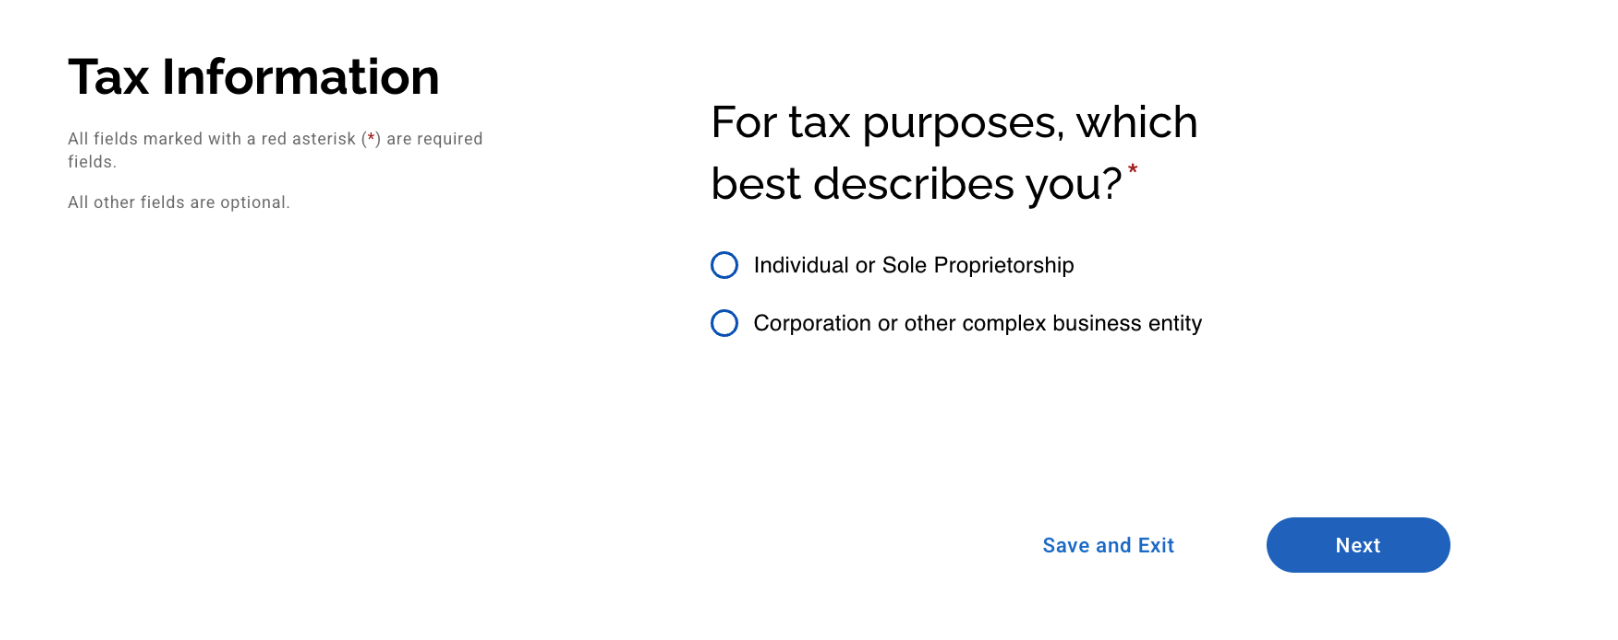
\includegraphics[keepaspectratio]{files/tax_info.png}}

\subsection{Provide your tax
information}\label{provide-your-tax-information}

\subsection{Generate Electronic W-9}\label{generate-electronic-w-9}

\begin{tcolorbox}[enhanced jigsaw, toptitle=1mm, colbacktitle=quarto-callout-note-color!10!white, opacitybacktitle=0.6, title=\textcolor{quarto-callout-note-color}{\faInfo}\hspace{0.5em}{Note}, leftrule=.75mm, left=2mm, rightrule=.15mm, coltitle=black, colframe=quarto-callout-note-color-frame, breakable, toprule=.15mm, opacityback=0, bottomtitle=1mm, colback=white, titlerule=0mm, arc=.35mm, bottomrule=.15mm]

If you are:

\begin{itemize}
\tightlist
\item
  a U.S. citizen, green card holder, or U.S. tax resident (resident
  alien), and
\item
  you have a valid SSN or EIN, and
\item
  you have \textbf{NOT} received any official notice from the IRS
  stating that you are subject to backup withholding,
\end{itemize}

then you may generally select:

\begin{itemize}
\tightlist
\item
  \textbf{Generate Electronic W-9} → \textbf{Yes}
\item
  \textbf{Backup Withholding} → leave this box checked
\item
  \textbf{Citizenship} → U.S. citizen or other U.S. person
\end{itemize}

\end{tcolorbox}

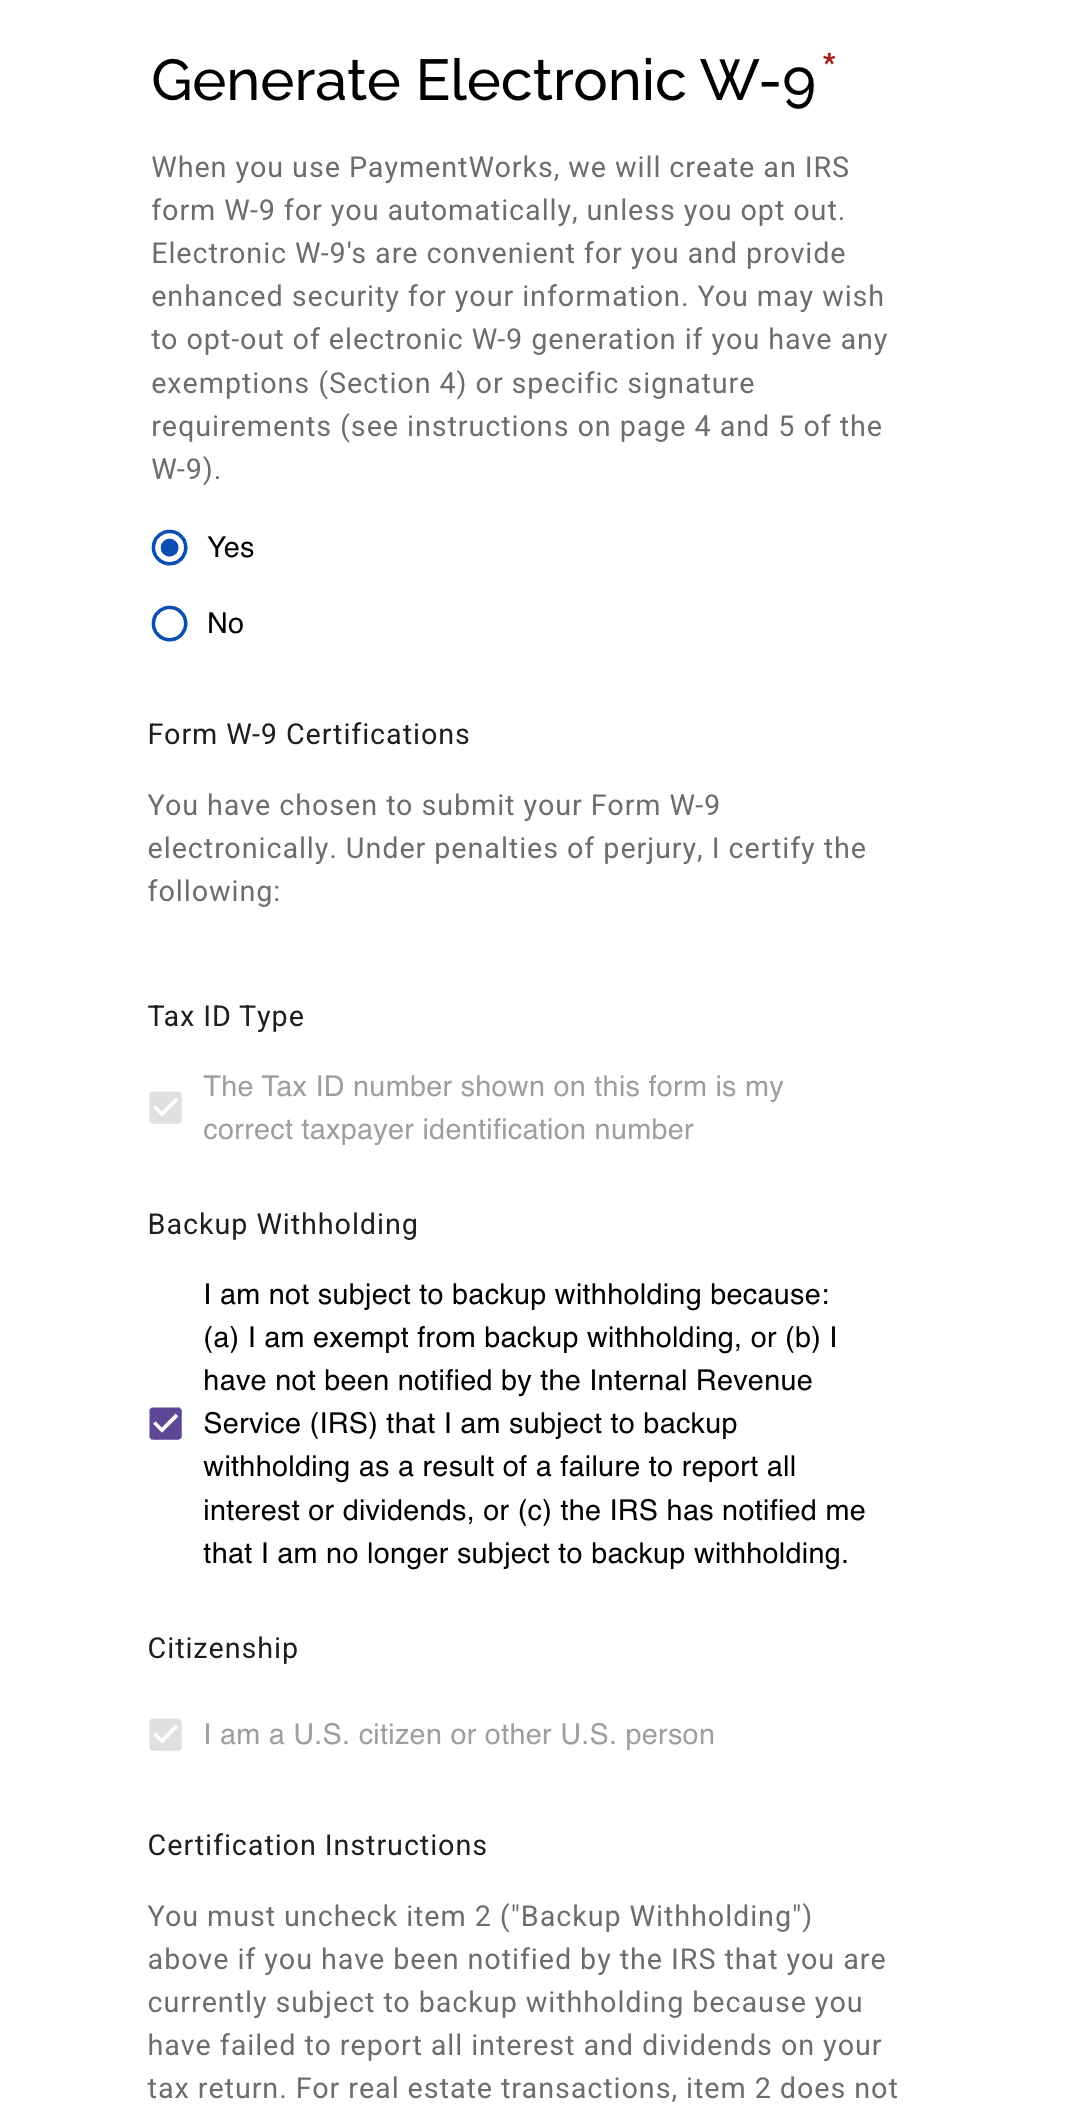
\includegraphics[width=1\linewidth,height=\textheight,keepaspectratio]{files/generate_w_9.png}

\subsection{Personal and Address
Information}\label{personal-and-address-information}

\begin{tcolorbox}[enhanced jigsaw, toptitle=1mm, colbacktitle=quarto-callout-note-color!10!white, opacitybacktitle=0.6, title=\textcolor{quarto-callout-note-color}{\faInfo}\hspace{0.5em}{Note}, leftrule=.75mm, left=2mm, rightrule=.15mm, coltitle=black, colframe=quarto-callout-note-color-frame, breakable, toprule=.15mm, opacityback=0, bottomtitle=1mm, colback=white, titlerule=0mm, arc=.35mm, bottomrule=.15mm]

\textbf{Remittance Address}:\\
Address where payment should be sent (e.g., check mailing address).

\end{tcolorbox}

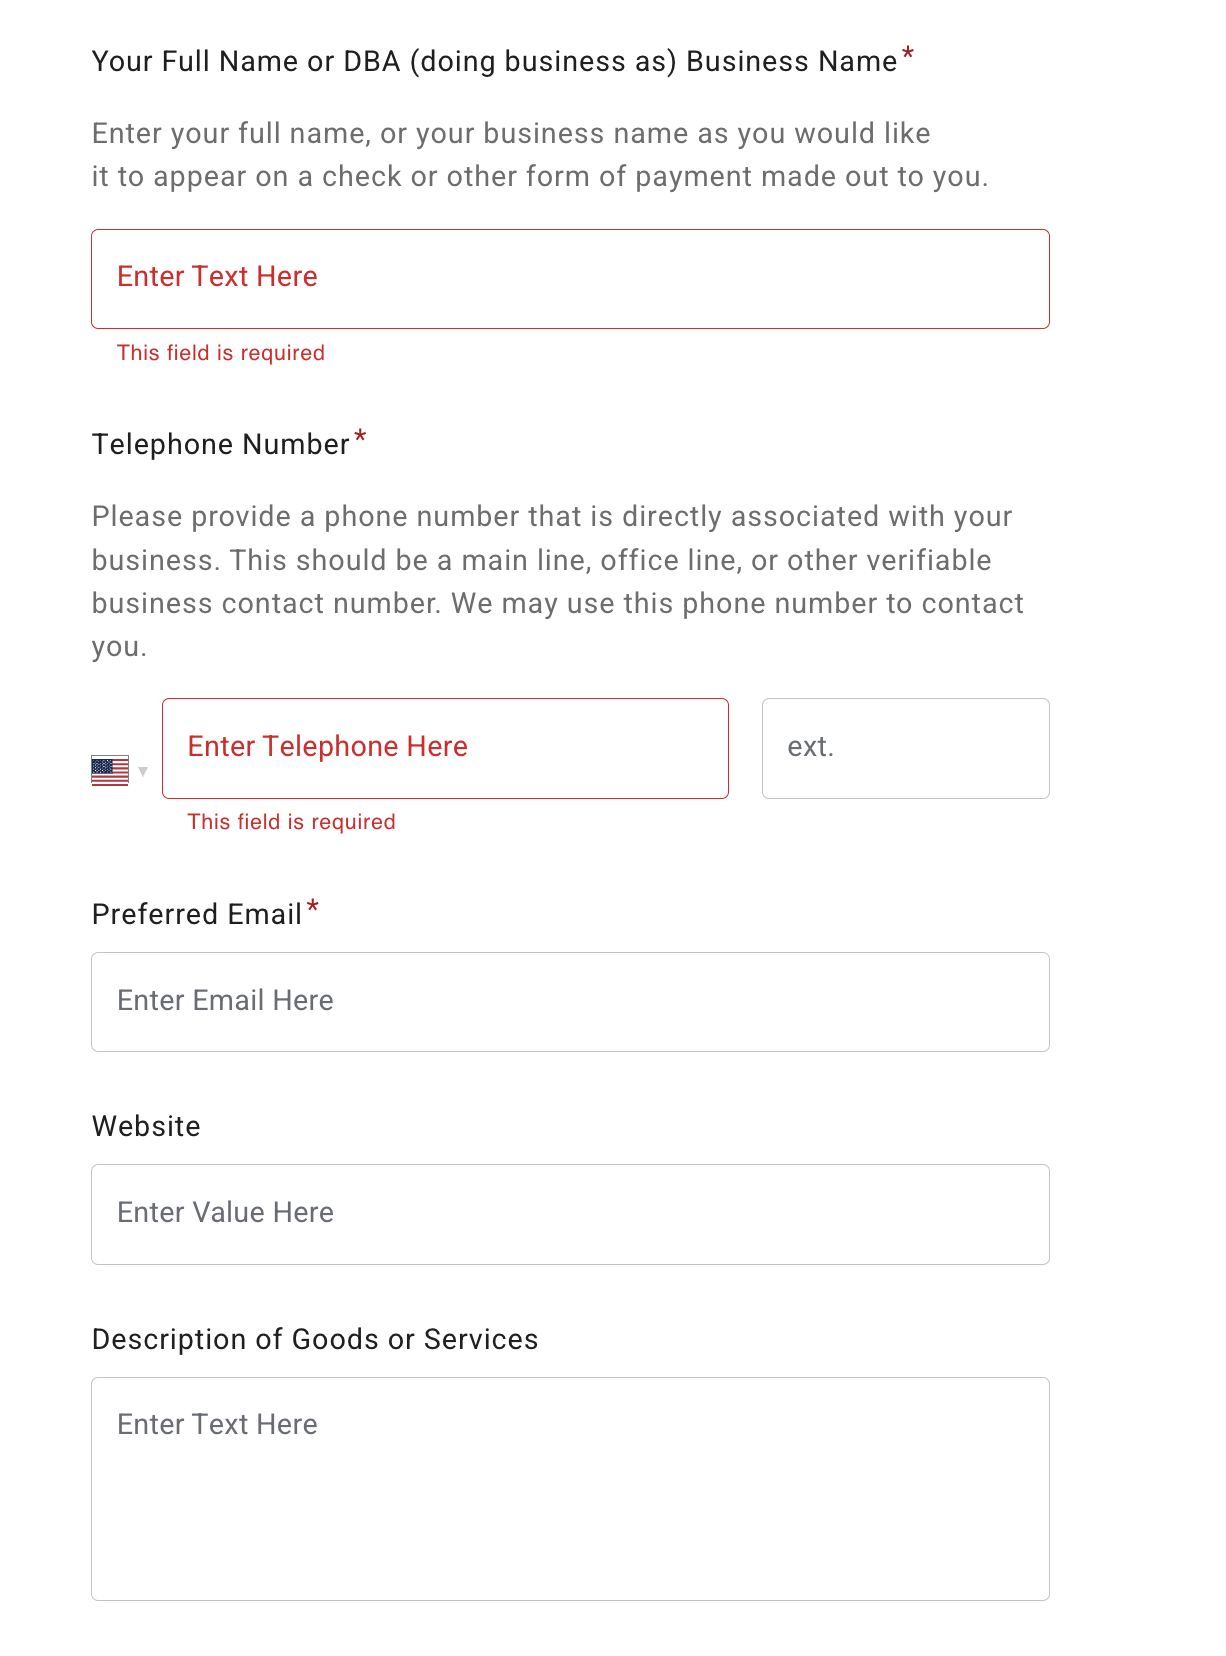
\includegraphics[width=1\linewidth,height=\textheight,keepaspectratio]{files/personal_info.png}

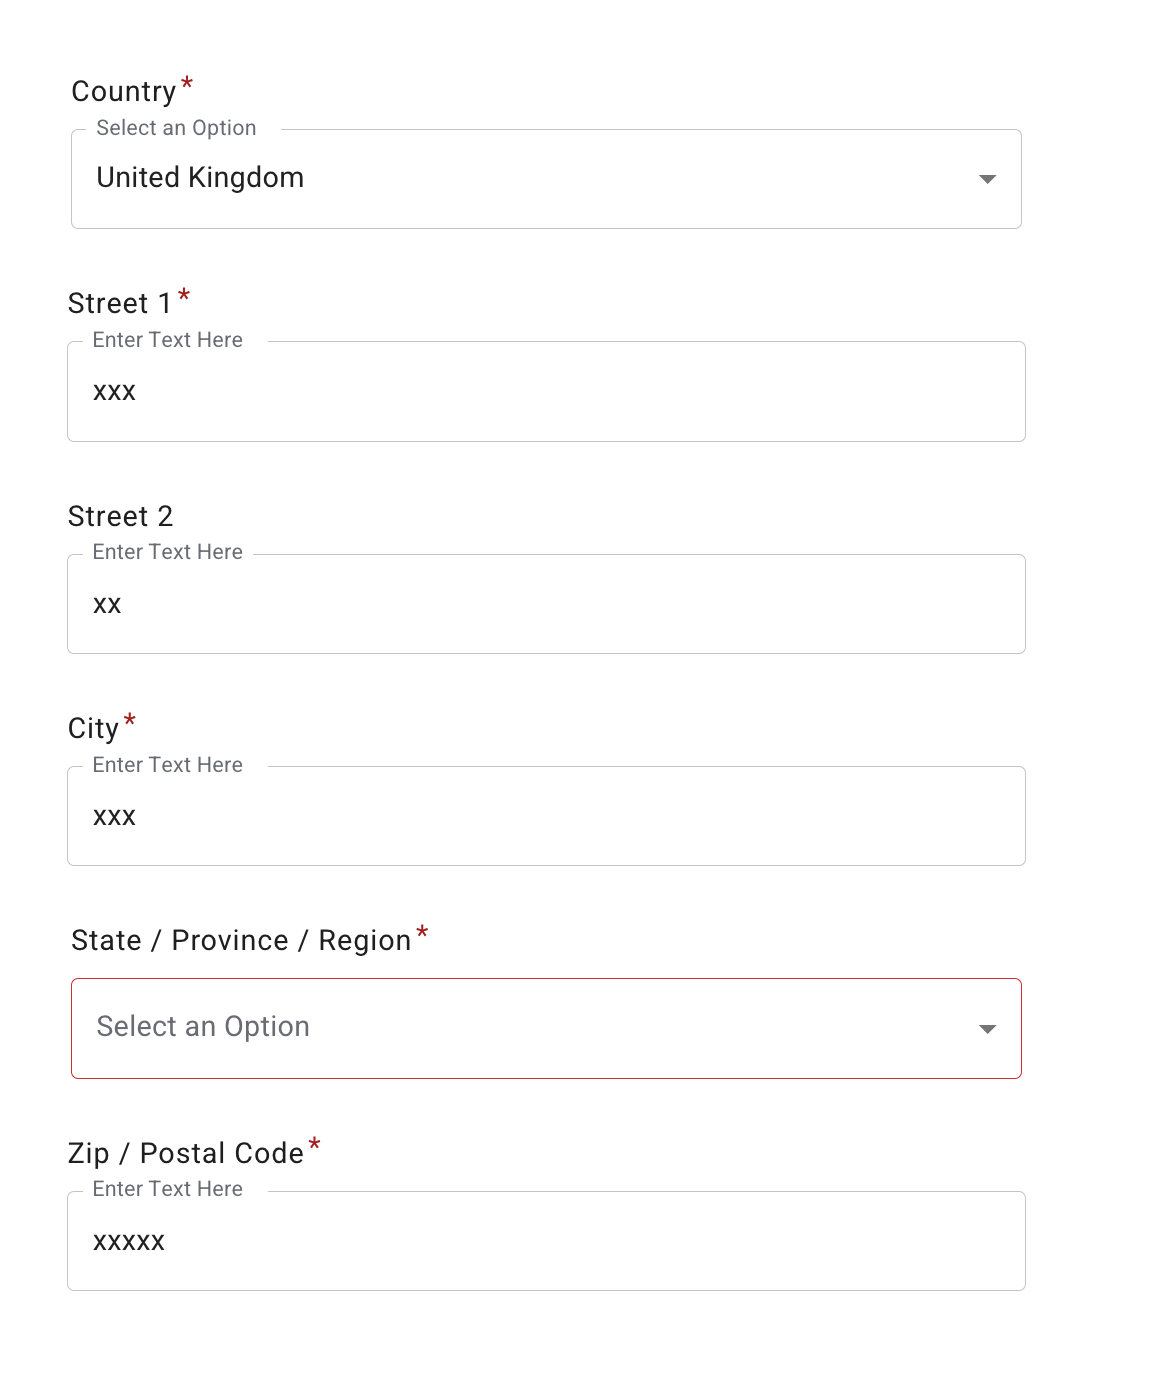
\includegraphics[width=1\linewidth,height=\textheight,keepaspectratio]{files/primary_address.png}

\subsection{Additional Information}\label{additional-information}

\begin{tcolorbox}[enhanced jigsaw, toptitle=1mm, colbacktitle=quarto-callout-note-color!10!white, opacitybacktitle=0.6, title=\textcolor{quarto-callout-note-color}{\faInfo}\hspace{0.5em}{Note}, leftrule=.75mm, left=2mm, rightrule=.15mm, coltitle=black, colframe=quarto-callout-note-color-frame, breakable, toprule=.15mm, opacityback=0, bottomtitle=1mm, colback=white, titlerule=0mm, arc=.35mm, bottomrule=.15mm]

\begin{itemize}
\tightlist
\item
  In general, you can simply complete it by following what is shown in
  the image.
\item
  If you are SDSU/SDSURF student or employee you will need to fill your
  sdsuid
\item
  These questions apply mainly to established businesses.

  \begin{itemize}
  \tightlist
  \item
    Do you accept credit cards?
  \item
    Do you accept Purchase Orders?\\
    Individuals can usually select \textbf{No}.
  \end{itemize}
\end{itemize}

\end{tcolorbox}

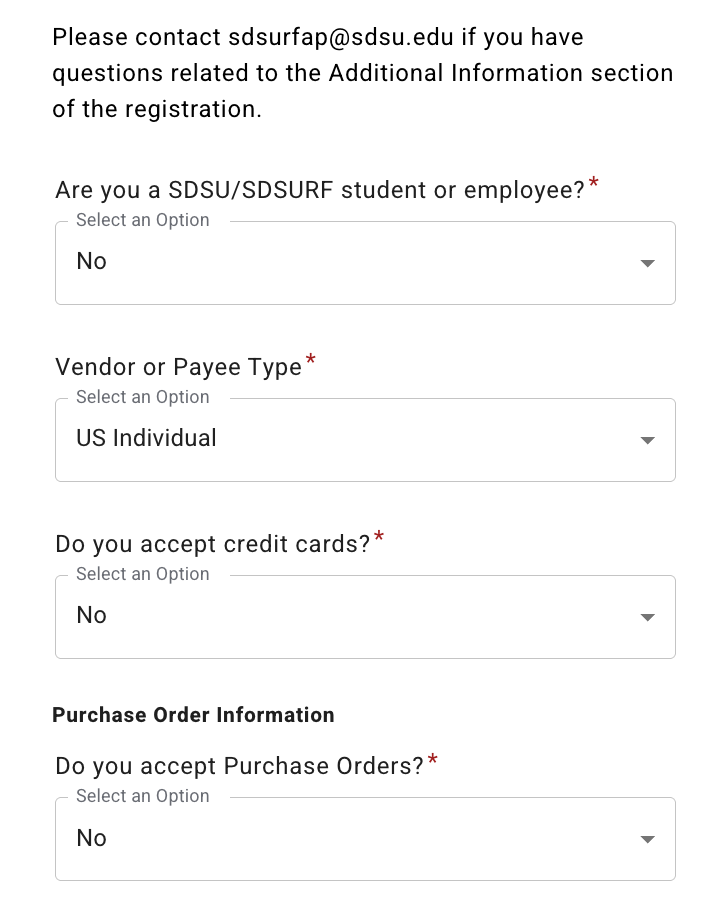
\includegraphics[width=1\linewidth,height=\textheight,keepaspectratio]{files/additional_info1.png}

\subsubsection{Conflict of interest}\label{conflict-of-interest}

\begin{tcolorbox}[enhanced jigsaw, toptitle=1mm, colbacktitle=quarto-callout-note-color!10!white, opacitybacktitle=0.6, title=\textcolor{quarto-callout-note-color}{\faInfo}\hspace{0.5em}{Note}, leftrule=.75mm, left=2mm, rightrule=.15mm, coltitle=black, colframe=quarto-callout-note-color-frame, breakable, toprule=.15mm, opacityback=0, bottomtitle=1mm, colback=white, titlerule=0mm, arc=.35mm, bottomrule=.15mm]

In general, choose \textbf{No} as most of us are just requesting travel
reimbursement.

\end{tcolorbox}

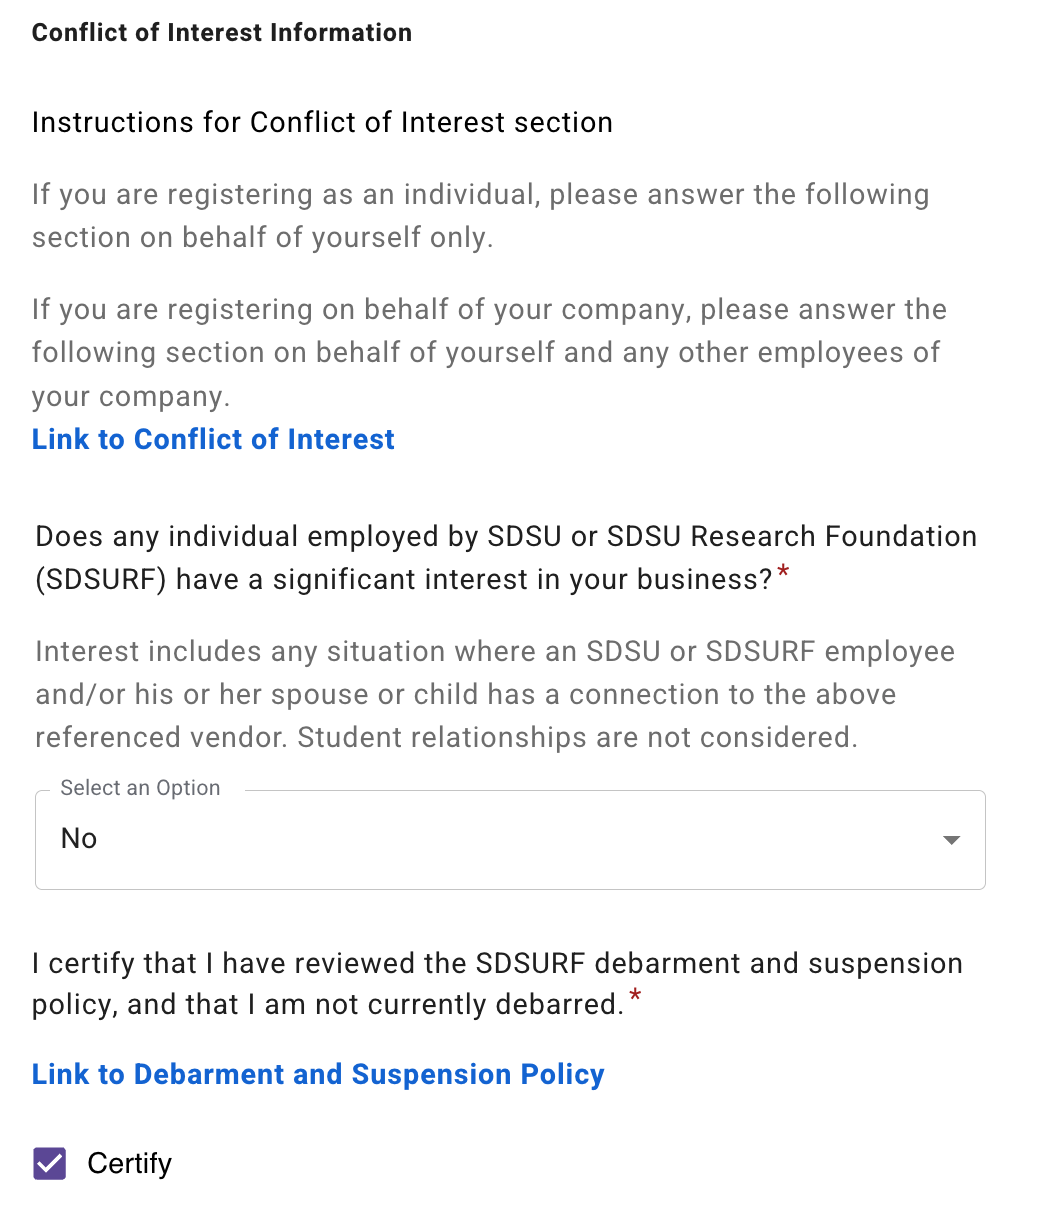
\includegraphics[width=1\linewidth,height=\textheight,keepaspectratio]{files/conflict_of_interest.png}

\subsubsection{Payment option}\label{payment-option}

\begin{tcolorbox}[enhanced jigsaw, toptitle=1mm, colbacktitle=quarto-callout-note-color!10!white, opacitybacktitle=0.6, title=\textcolor{quarto-callout-note-color}{\faInfo}\hspace{0.5em}{Note}, leftrule=.75mm, left=2mm, rightrule=.15mm, coltitle=black, colframe=quarto-callout-note-color-frame, breakable, toprule=.15mm, opacityback=0, bottomtitle=1mm, colback=white, titlerule=0mm, arc=.35mm, bottomrule=.15mm]

ACH is recommended for direct deposit to your bank account.

\end{tcolorbox}

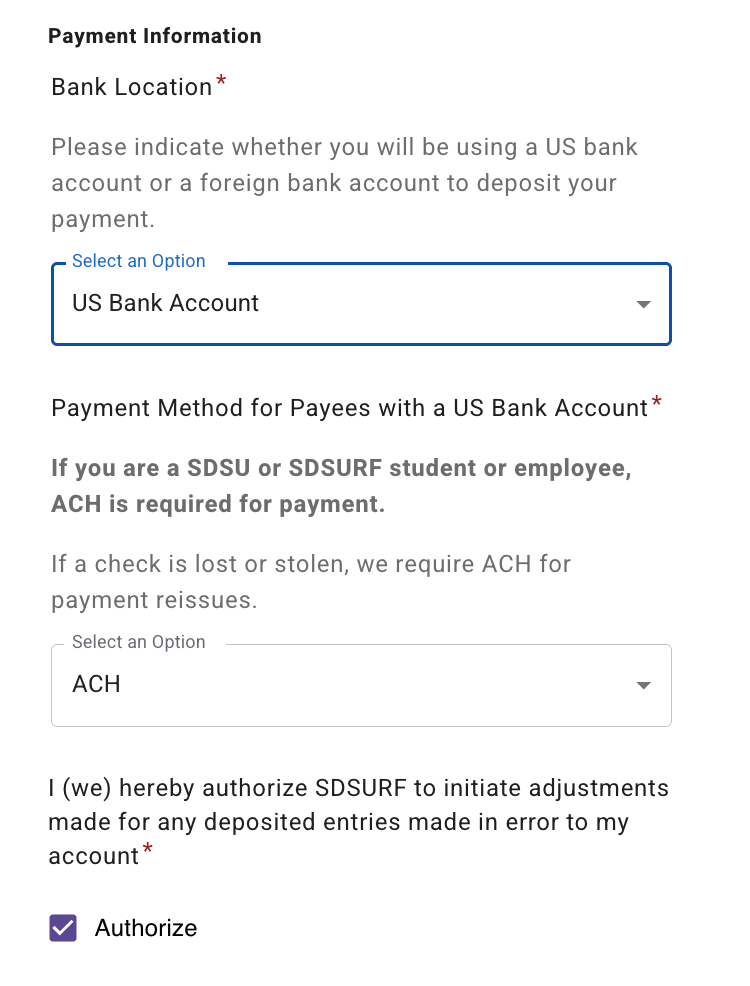
\includegraphics[width=1\linewidth,height=\textheight,keepaspectratio]{files/payment_us.png}

\subsection{Provide Your Bank
Information}\label{provide-your-bank-information}

\begin{tcolorbox}[enhanced jigsaw, toptitle=1mm, colbacktitle=quarto-callout-note-color!10!white, opacitybacktitle=0.6, title=\textcolor{quarto-callout-note-color}{\faInfo}\hspace{0.5em}{Note}, leftrule=.75mm, left=2mm, rightrule=.15mm, coltitle=black, colframe=quarto-callout-note-color-frame, breakable, toprule=.15mm, opacityback=0, bottomtitle=1mm, colback=white, titlerule=0mm, arc=.35mm, bottomrule=.15mm]

The backup document is used to verify that the information entered on
the registration form is accurate.\\
A document that includes \textbf{your bank routing number} and
\textbf{your full bank account number} is preferred.

\end{tcolorbox}

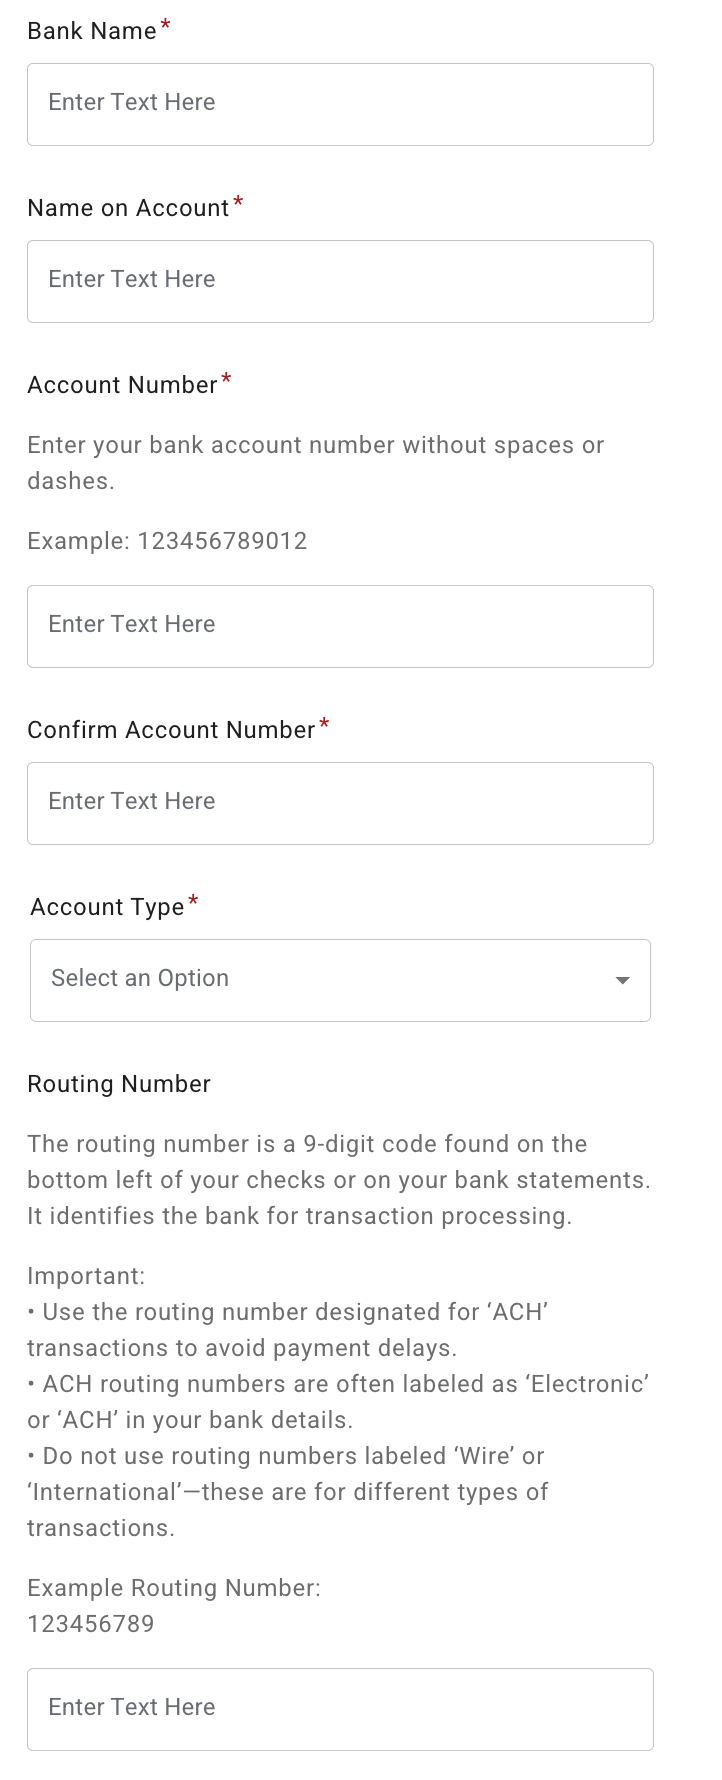
\includegraphics[width=1\linewidth,height=\textheight,keepaspectratio]{files/bank_info.png}

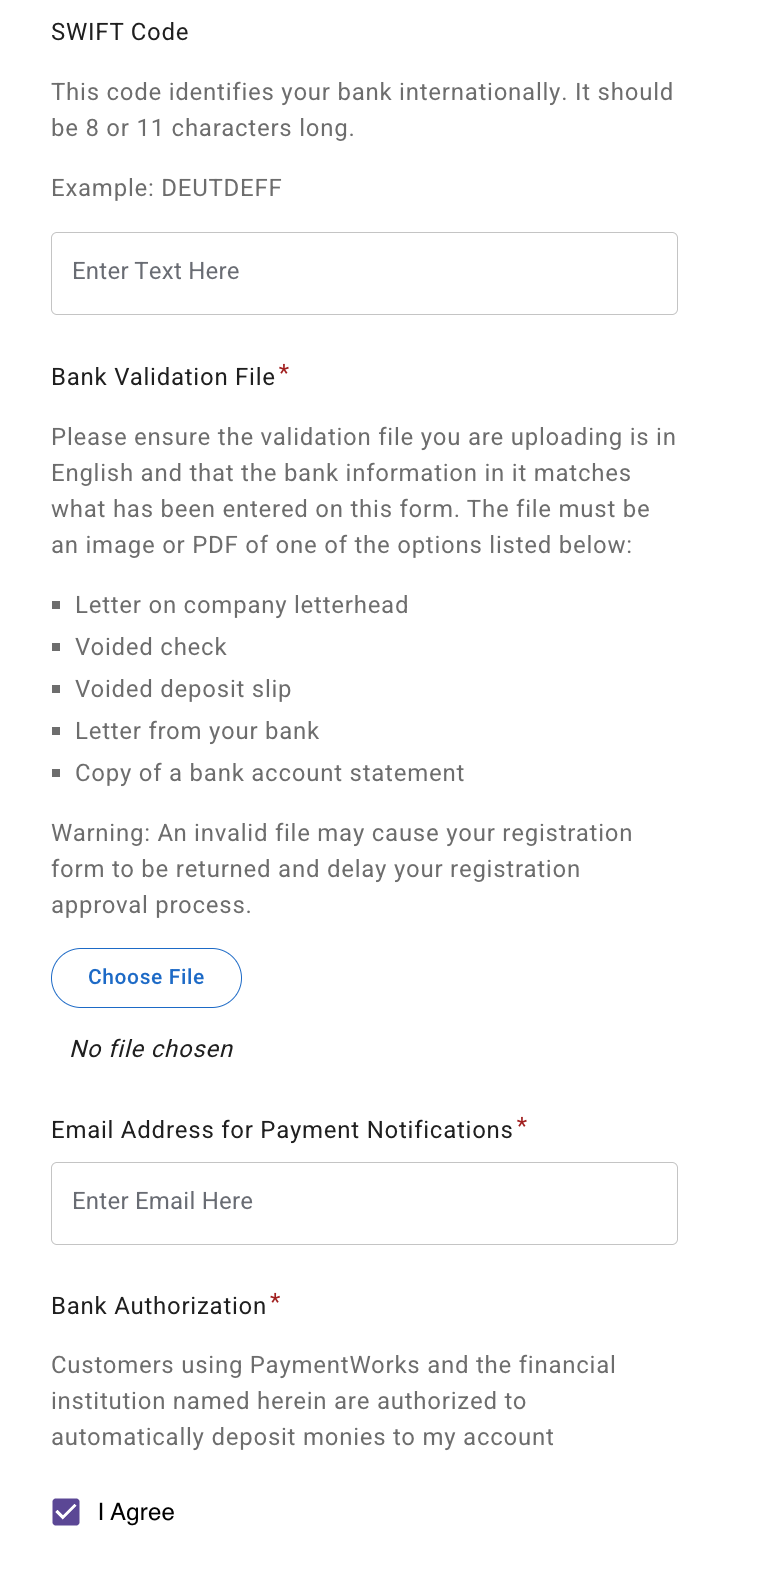
\includegraphics[width=1\linewidth,height=\textheight,keepaspectratio]{files/bank_info2.png}

\subsubsection{Bank Address Information}\label{bank-address-information}

\begin{tcolorbox}[enhanced jigsaw, toptitle=1mm, colbacktitle=quarto-callout-note-color!10!white, opacitybacktitle=0.6, title=\textcolor{quarto-callout-note-color}{\faInfo}\hspace{0.5em}{Note}, leftrule=.75mm, left=2mm, rightrule=.15mm, coltitle=black, colframe=quarto-callout-note-color-frame, breakable, toprule=.15mm, opacityback=0, bottomtitle=1mm, colback=white, titlerule=0mm, arc=.35mm, bottomrule=.15mm]

The bank address does not have to be the branch where you originally
opened your account.\\
For example, if your bank account is with \textbf{Chase}, you may enter
the address of \textbf{any Chase branch that is close to you}.

\end{tcolorbox}

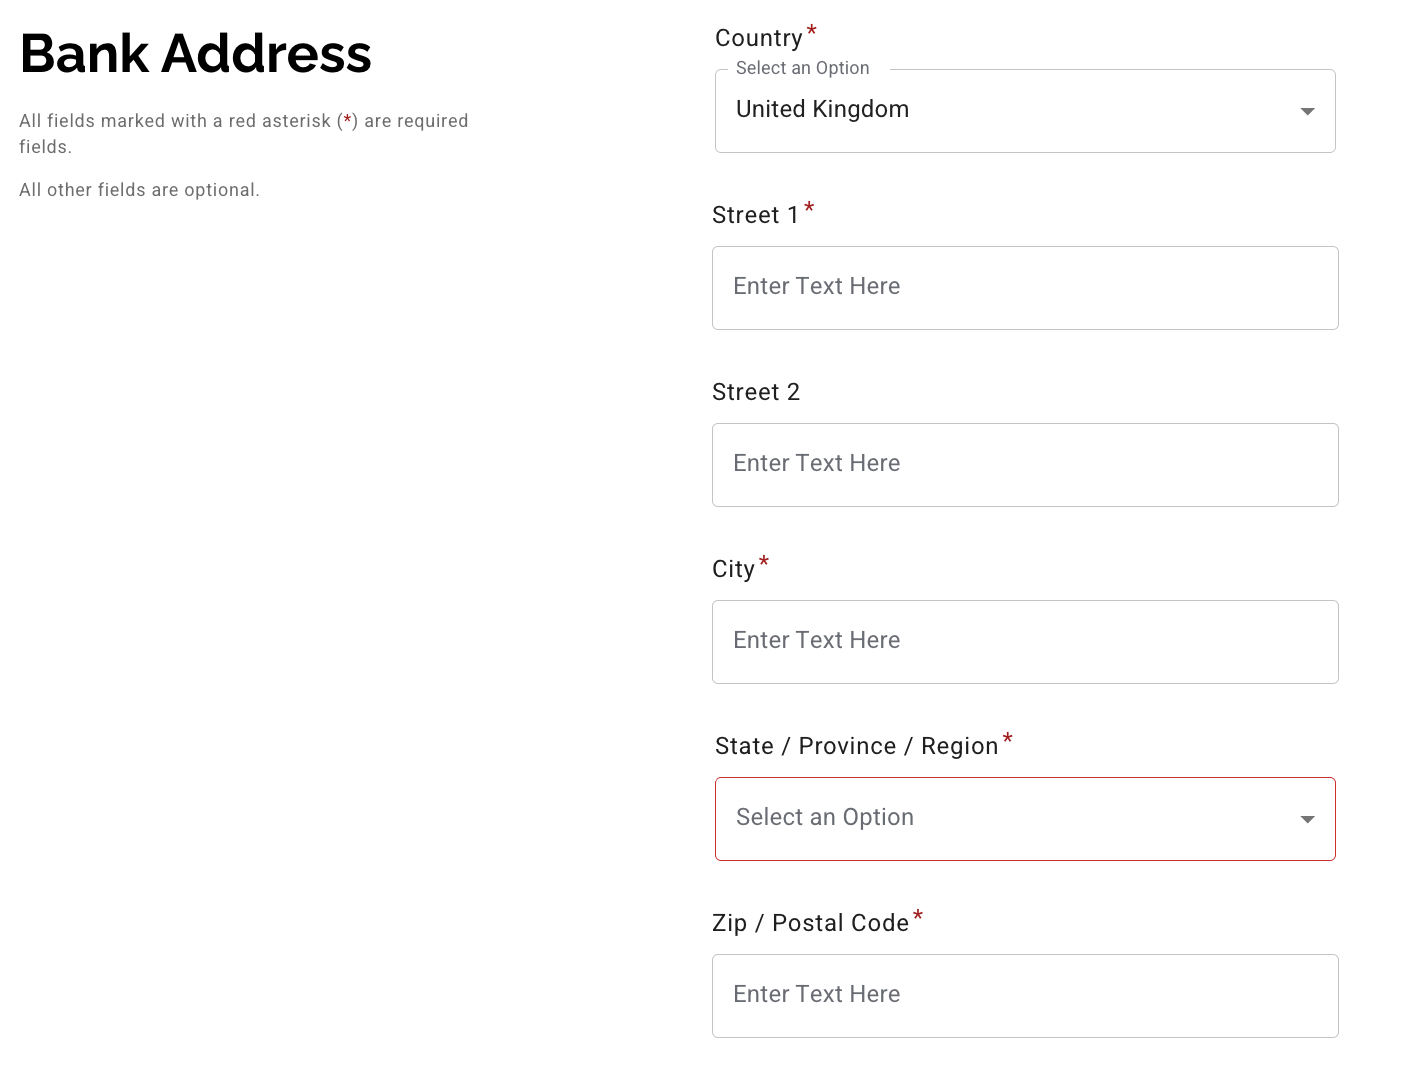
\includegraphics[width=1\linewidth,height=\textheight,keepaspectratio]{files/bank_info3.png}




\end{document}
